\documentclass[pdftex,12pt,a4paper]{article}

\usepackage{graphicx}  
\usepackage[margin=2.5cm]{geometry}
\usepackage{breakcites}
\usepackage{indentfirst}
\usepackage{pgfgantt}
\usepackage{pdflscape}
\usepackage{float}
\usepackage{epsfig}
\usepackage{epstopdf}
\usepackage[cmex10]{amsmath}
\usepackage{stfloats}
\usepackage{multirow}
\usepackage{karnaugh-map}

\renewcommand{\refname}{REFERENCES}
\linespread{1.3}

\usepackage{mathtools}
%\newcommand{\HRule}{\rule{\linewidth}{0.5mm}}
\thispagestyle{empty}
\begin{document}
\begin{titlepage}
\begin{center}
\textbf{}\\
\textbf{\Large{ISTANBUL TECHNICAL UNIVERSITY}}\\
\vspace{0.5cm}
\textbf{\Large{COMPUTER ENGINEERING DEPARTMENT}}\\
\vspace{2cm}
\textbf{\Large{BLG 242E\\ DIGITAL CIRCUITS LABORATORY\\ EXPERIMENT REPORT}}\\
\vspace{2.8cm}
\begin{table}[ht]
\centering
\Large{
\begin{tabular}{lcl}
\textbf{EXPERIMENT NO}  & : & 3 \\
\textbf{EXPERIMENT DATE}  & : & 01.03.2019 \\
\textbf{LAB SESSION}  & : & FRIDAY - 14.00 \\
\textbf{GROUP NO}  & : & G13 \\
\end{tabular}}
\end{table}
\vspace{1cm}
\textbf{\Large{GROUP MEMBERS:}}\\
\begin{table}[ht]
\centering
\Large{
\begin{tabular}{rcl}
{
150180704  & : & C\.{I}HAT AKK\.{I}RAZ \\
150180707  & : & FAT\.{I}H ALTINPINAR \\
150180734  & : & S\.{I}NAN \c{S}AR \\
}
\end{tabular}}
\end{table}
\vspace{2.8cm}
\textbf{\Large{SPRING 2019}}

\end{center}

\end{titlepage}

\newpage

\thispagestyle{empty}
\centering{\LARGE{ \textbf{ETHIC FORM}}}\\
\centering{\LARGE{\textbf{for}}}\\
\centering{\LARGE{\textbf{BLG242E Logic Circuits Laboratory}}}\\[0.2cm]
As a student of \\Istanbul Technical University Faculty of Computer and Informatics Engineering;
\begin{enumerate}
    \item I will not attempt to cheat in quizes and final exam,
    \item I will not use disallowed sources or tools (mobile phone, calculator etc.) during the exam,
    \item I will not write any information (formula, text, figure etc.) on the table, sheets or books that are allowed to be used during the exam,
    \item I will give reference when using printed or online published sources,
    \item I will not use the results in a source as they are, or by changing a part of them without giving a reference,
    \item I will not show unused sources as used, 
    \item I will not present someone else’s idea as my own idea, 
    \item I will not make someone do my homework, project or thesis for money or anything else,
    \item I will not take an exam or enter a lecture on behalf of others,
    \item I will not make excuses for not attending in exams or lessons by taking reports from someone I know (medical doctor parents or relatives),
    \item I will refrain from deliberately harming the public materials at our university,  
    \item I will comply with the safety rules in laboratory work,
    \item I will behave in accordance with the rules of respect for the lecturers and teaching assistants
\end{enumerate}
\vspace{-1em}
\centering{\LARGE{signed by}}\\
\vspace{-1em}
\begin{table}[ht]
\centering
\begin{tabular}{rcl}
150180704  & : & C\.{I}HAT AKK\.{I}RAZ \\
150180707  & : & FAT\.{I}H ALTINPINAR \\
150180734  & : & S\.{I}NAN \c{S}AR \\
\end{tabular}
\end{table}
\vspace{-1em}
 \begin{table}[ht]
 \begin{tabular}{lr}
%\textbf{Date:\hspace*{1.0cm}/\hspace*{1.0cm}/} &\qquad \qquad\qquad\qquad \qquad\qquad\qquad \qquad\qquad\qquad \qquad\qquad \textbf{SIGNED}\\
\end{tabular}
\end{table} % adds the ethic sign
\addcontentsline{toc}{section}{\numberline {}ETHICS}
\newpage

\thispagestyle{empty}
\addtocontents{toc}{\contentsline {section}{\numberline {}FRONT COVER}{}}
\addtocontents{toc}{\contentsline {section}{\numberline {}CONTENTS}{}}
\setcounter{tocdepth}{4}
\tableofcontents
\clearpage

\setcounter{page}{1}

\section{INTRODUCTION}
\begin{flushleft}
\paragraph{}
In this experiment we have tried to find prime implicants of some functions and implement them with the lowest cost possible, using combinational logic circuits, NOT, AND, OR, NAND, NOR gates, a decoder and a multiplexer provided to us.
%cool!!
\end{flushleft}

\section{REQUIREMENTS}
\begin{flushleft}
\underline{Tools Used}\cite{booklet}
\end{flushleft}
\begin{itemize}
    \item C.A.D.E.T
    \item 74000 series ICs
    \begin{itemize}
        \item 74xx00 - Quadruple 2-input Positive NAND Gates
        \item 74xx04 - Hex Inverters     
        \item 74xx08 - Quadruple 2-input Positive AND Gates
        \item 74xx10 - Triple 3-input Positive NAND Gates
        \item 74xx11 - Triple 3-input Positive AND Gates
        \item 74xx27 - Triple 3-input Positive NOR Gates
        \item 74xx32 - Quadruple 2-input Positive OR Gates
        \item 74xx138 - 3:8 Decoder
        \item 74xx151 - 8:1 Multiplexer
    \end{itemize}
\end{itemize}
\begin{flushleft}
\subsection{PART 1}

%\begin{figure}[ht]
%	\centering
%	
\includegraphics[width=0.5\textwidth]{logo.png}	
%	\caption{An Example Figure Caption\cite{ref1}}
%	\label{fig1}
%\end{figure}


\paragraph{}
In this part, the circuit is designed for the given function (The function can be seen below). Before building the circuit, its karnaugh diagram is created to find the essential prime implicants of the function. Sum of essential prime implicants gives the expression with minimum cost. The circuit is implemented by using AND, OR and NOT gates. Connections between pins are made for each integrated circuits as needed, outputs ae observed on the logic monitor.

\begin{itemize}
    \item $F_{1}$(a,b,c,d) = $U_{1}$(0, 3, 5, 7, 11, 12, 13) + $U_{\Phi}$(1, 8, 15)  
\end{itemize}

\paragraph{}
While finding essential prime implicants don't care($\Phi$) input values are considered as true(1), while creating the prime implicant chart, they are considered as false(0).


\newpage

\begin{figure}[!h]
\begin{karnaugh-map}[4][4][1][$c d$][$a b$]
\minterms{0,3,5,7,11,12,13}
\terms{1,8,15}{${\Phi}$}
\terms{2,4,6,9,10,14}{0}
\implicant{0}{1}
\implicant{3}{11}
\implicant{12}{8}
\implicant{5}{15}
\implicant{1}{7}
\implicant{12}{13}
\implicantedge{0}{8}

\end{karnaugh-map}
\centering
\caption{Karnaugh map of $F$}
\label{karnaugh1}
\end{figure}




\begin{table}[h]
\begin{tabular}{ccccccc}
              & $c \cdot d$  & $a' \cdot d$ & $b \cdot d$ & $a' \cdot b' \cdot c'$ & $a \cdot b \cdot c'$ & $a \cdot c' \cdot d'$ \\
SYMBOL         & A            & B            & C           & D                      & E                    & F                     \\
COST           & 4            & 5            & 4           & 9                      & 7                    & 8                     \\
COVERED POINTS & 3, 7, 11, 15 & 3, 5, 7      & 5, 7, 13    & 0                      & 12, 13               & 12                   
\end{tabular}

\caption{All prime implicants}
\label{ponisandta}
\end{table}



\begin{flushleft}
\paragraph{}
After labeling, prime implicant chart is formed by putting a prime implicant on a row and marking every point that covered by that prime implicant. 
\end{flushleft}



\begin{table}[h]
\centering
\begin{tabular}{l|l|l|l|l|l|l|l|l|}
\cline{2-9}
                        & 0                        & 3 & 5 & 7 & 11                       & 12 & 13                       & COST \\ \hline
\multicolumn{1}{|l|}{A} &                          & x &   & x & {\color[HTML]{FE0000} x} &    &                          & 4    \\ \hline
\multicolumn{1}{|l|}{B} &                          & x & x & x &                          &    &                          & 5    \\ \hline
\multicolumn{1}{|l|}{C} &                          &   & x & x &                          &    & {\color[HTML]{FE0000} x} & 4    \\ \hline
\multicolumn{1}{|l|}{D} & {\color[HTML]{FE0000} x} &   &   &   &                          &    &                          & 9    \\ \hline
\multicolumn{1}{|l|}{E} &                          &   &   &   &                          & x  & x                        & 7    \\ \hline
\multicolumn{1}{|l|}{F} &                          &   &   &   &                          & x  &                          & 12   \\ \hline
\end{tabular}
\caption{Prime implicant chart. Distinguished points are shown as red.}
\label{primeimplicantchart}
\end{table}

\begin{flushleft}
\paragraph{}
As we can see in the prime implicant chart(Table 2) distinguished points are shown as red. Prime implicants that are covering these points must be chosen. Therefore we chose A,C and D then remove them from the chart. We also remove any column that is covered by these prime implicants.
\end{flushleft}



\newpage


\begin{table}[h]
\centering
\begin{tabular}{c|c|c|}
\cline{2-3}
                        & 12 & COST \\ \hline
\multicolumn{1}{|c|}{E} & x  & 7    \\ \hline
\multicolumn{1}{|c|}{F} & x  & 12   \\ \hline
\end{tabular}
\caption{Implicant chart after removing A,C and D and colums covered by them.}
\label{primeimplicantchart2}
\end{table}

\begin{flushleft}
\paragraph{}
After removing A,D and C from the prime implicant chart we are left with E and F(Table 3). Since E covers the point that is covered by F and costs less we chose E as the final prime implicant. There is no point left to be covered.
\end{flushleft}



\begin{figure}[!h]
\begin{karnaugh-map}[4][4][1][$c d$][$a b$]
\minterms{0,3,5,7,11,12,13}
\terms{1,8,15}{${\Phi}$}
\terms{2,4,6,9,10,14}{0}
\implicant{0}{1}
\implicant{3}{11}
\implicant{12}{8}
\implicant{5}{15}
\end{karnaugh-map}
\centering
\caption{Chosen prime implicants on the Karnaugh map.}
\label{karnaugh3}
\end{figure}



\paragraph{}
Thus we get the F function as:

\begin{itemize}
    \item F(a,b,c) = $a' \cdot b' \cdot c' + a \cdot b \cdot c' + b \cdot d + c \cdot d$ 
\end{itemize}

%F = A'B'C' + ABC' + BD + CD



\begin{figure}[!h]
	\centering
	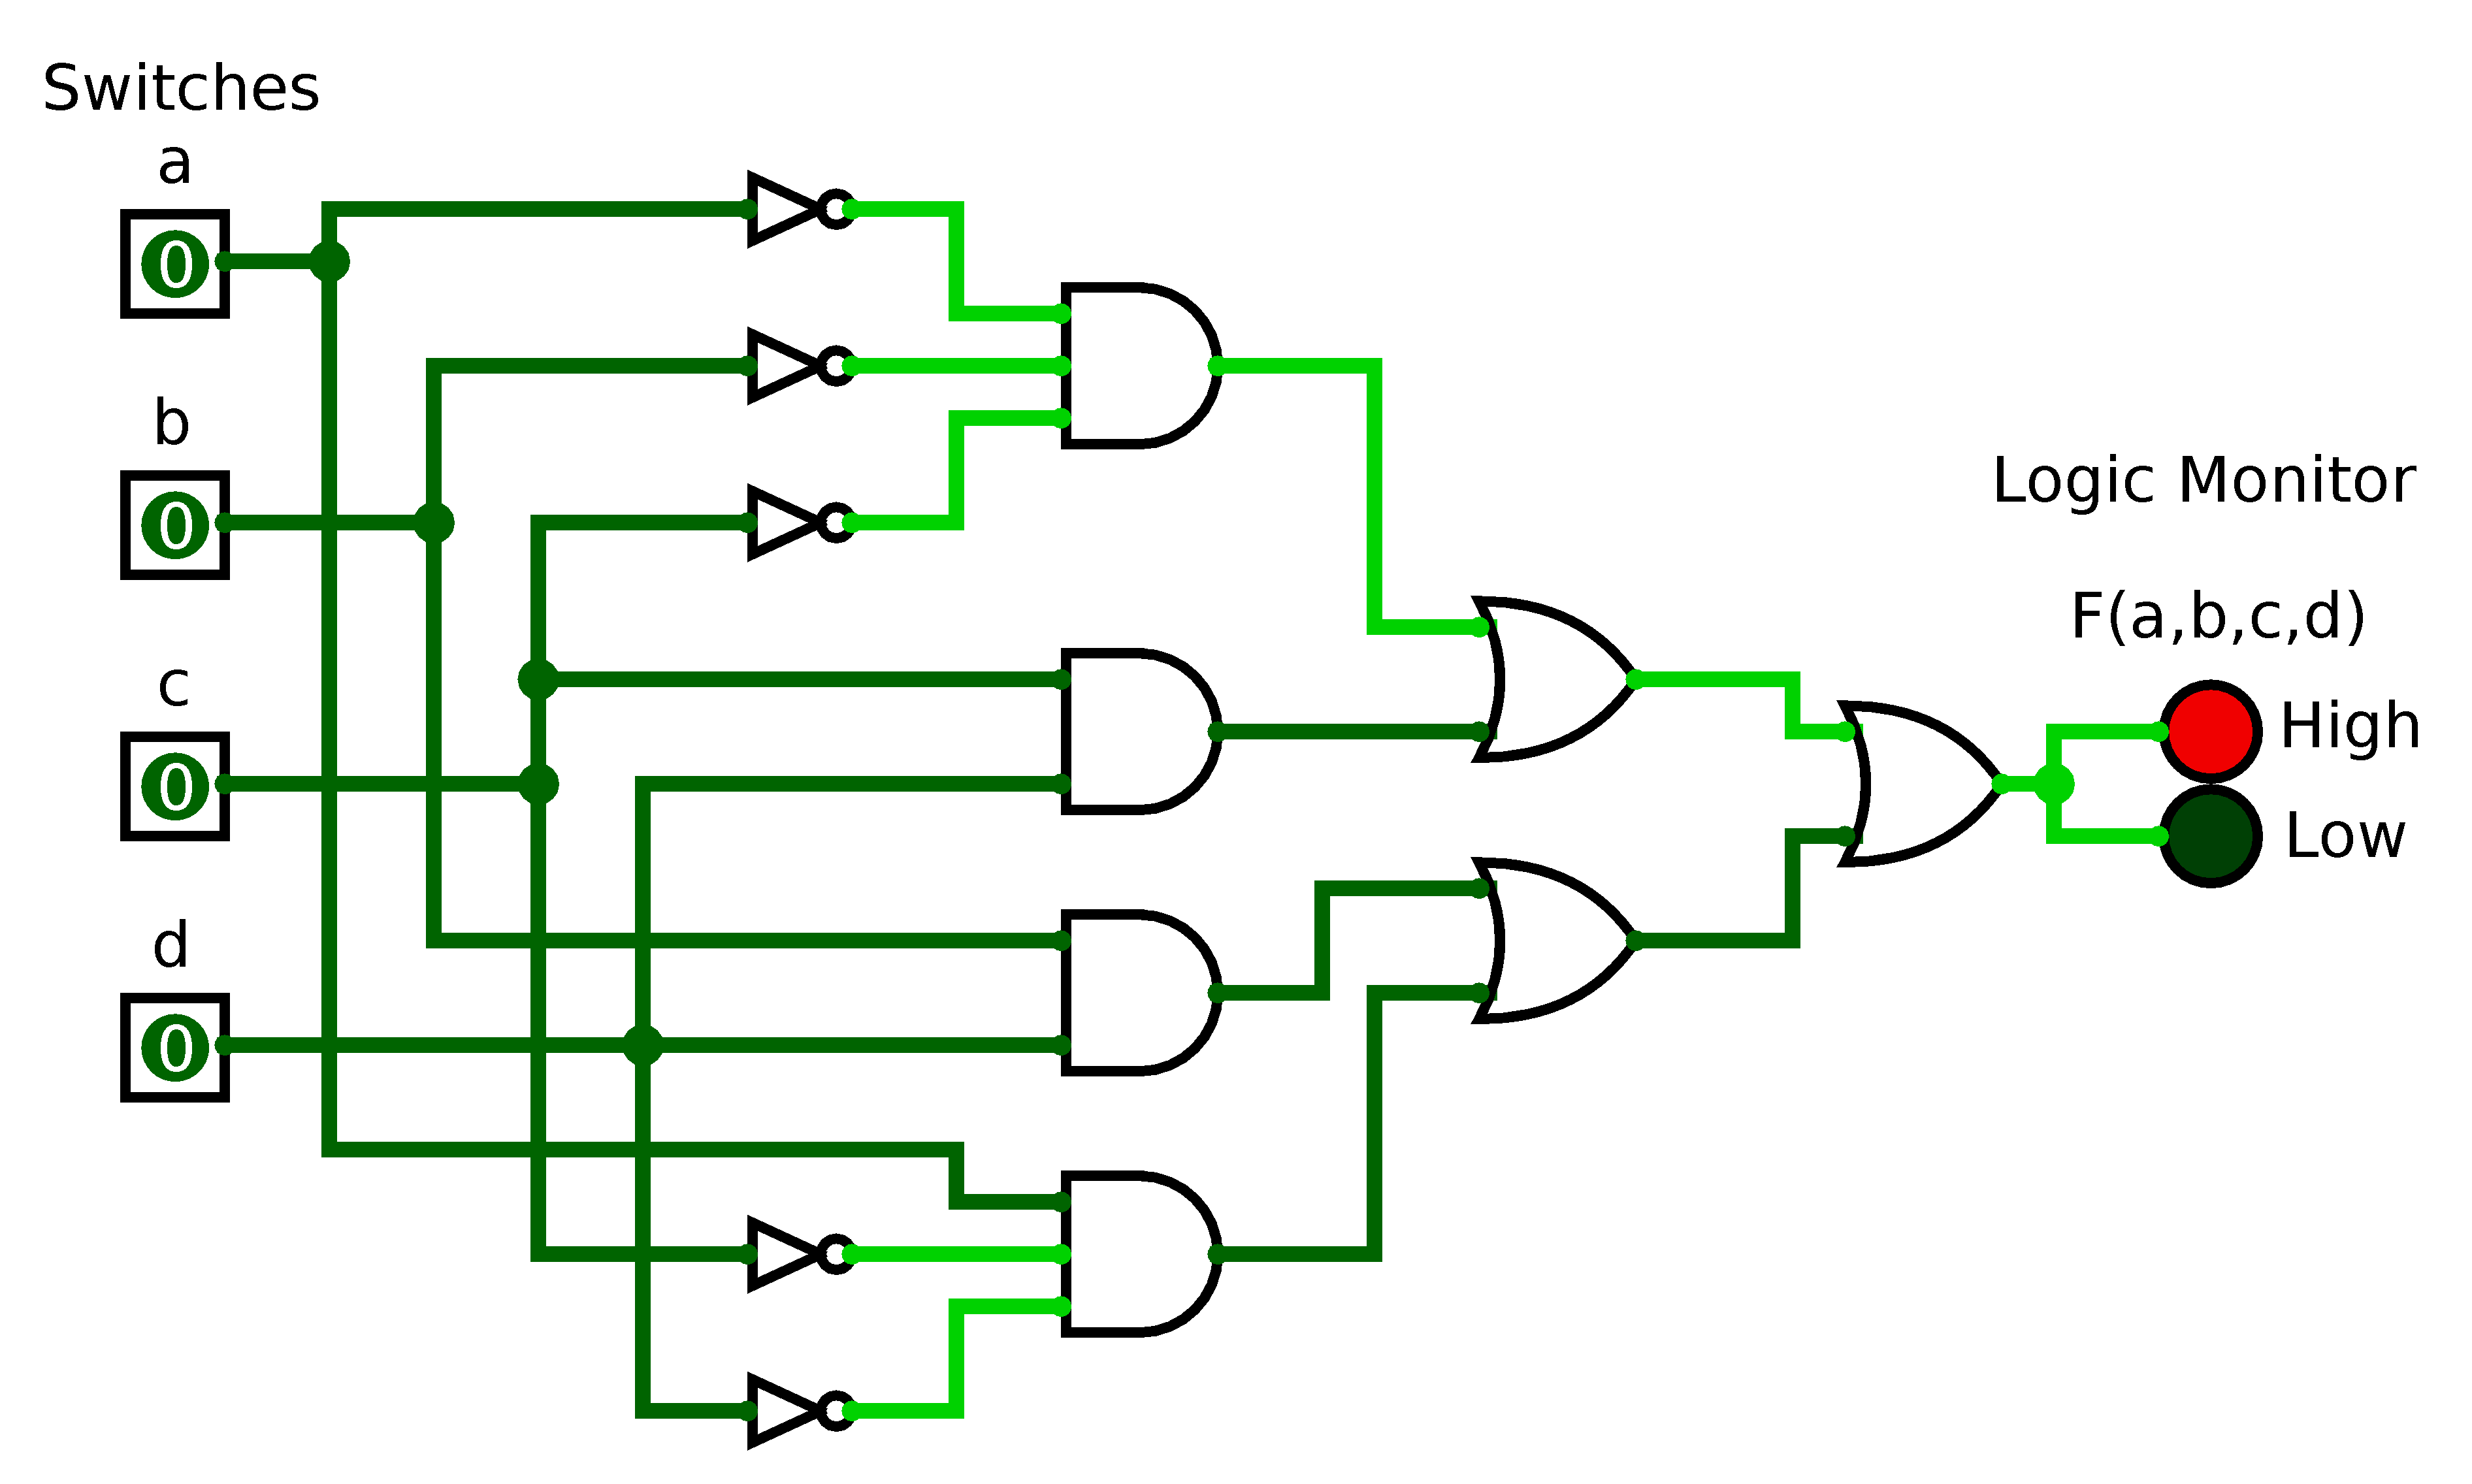
\includegraphics[width=0.5\textwidth]{part1.png}	
	\caption{Circuit of $F(a,b,c,d)$}
	\label{fig1}
\end{figure}

\begin{table}[!h]
\begin{center}
    \begin{tabular}{|c|c|c|c|c|c|}
    \hline
         A & B & C & D & F \\
         \hline
         0 & 0 & 0 & 0 & 1 \\
         \hline
         0 & 0 & 0 & 1 & ${\Phi}$ \\
         \hline
         0 & 0 & 1 & 0 & 0 \\
         \hline
         0 & 0 & 1 & 1 & 1 \\
         \hline
         0 & 1 & 0 & 0 & 0 \\
         \hline
         0 & 1 & 0 & 1 & 1 \\
         \hline
         0 & 1 & 1 & 0 & 0 \\
         \hline
         0 & 1 & 1 & 1 & 1 \\
         \hline
         1 & 0 & 0 & 0 & ${\Phi}$ \\
         \hline
         1 & 0 & 0 & 1 & 0 \\
         \hline
         1 & 0 & 1 & 0 & 0 \\
         \hline
         1 & 0 & 1 & 1 & 1 \\
         \hline
         1 & 1 & 0 & 0 & 1 \\
         \hline
         1 & 1 & 0 & 1 & 1 \\
         \hline
         1 & 1 & 1 & 0 & 0 \\
         \hline
         1 & 1 & 1 & 1 & ${\Phi}$ \\
         \hline
    \hline
    \end{tabular}
    \caption{Truth table of the given expression.}
    \label{truthtablep1}
\end{center}
\end{table}

\paragraph{}
The output values of the circuit are validated with the truth table above. If a don't care points manages to get into a prime implicant (as it can be seen in Figure 2) it gives an output of 1 otherwise 0. But we simply don't care it's value.
% The output values of the circuit are validated with the truth table above. When the input values are don't care, a random result appears and we simply don't care about it's value.
\end{flushleft}

\begin{flushleft}
\newpage
\subsection{PART 2}
\paragraph{}
In the second part of the experiment, same circuit is implemented using only NAND and NOT gates. Connections between pins are made for each integrated circuits as needed, outputs are observed on the logic monitor. The output values of the circuit are validated with the truth table in the part 1. 

\begin{figure}[!h]
	\centering
	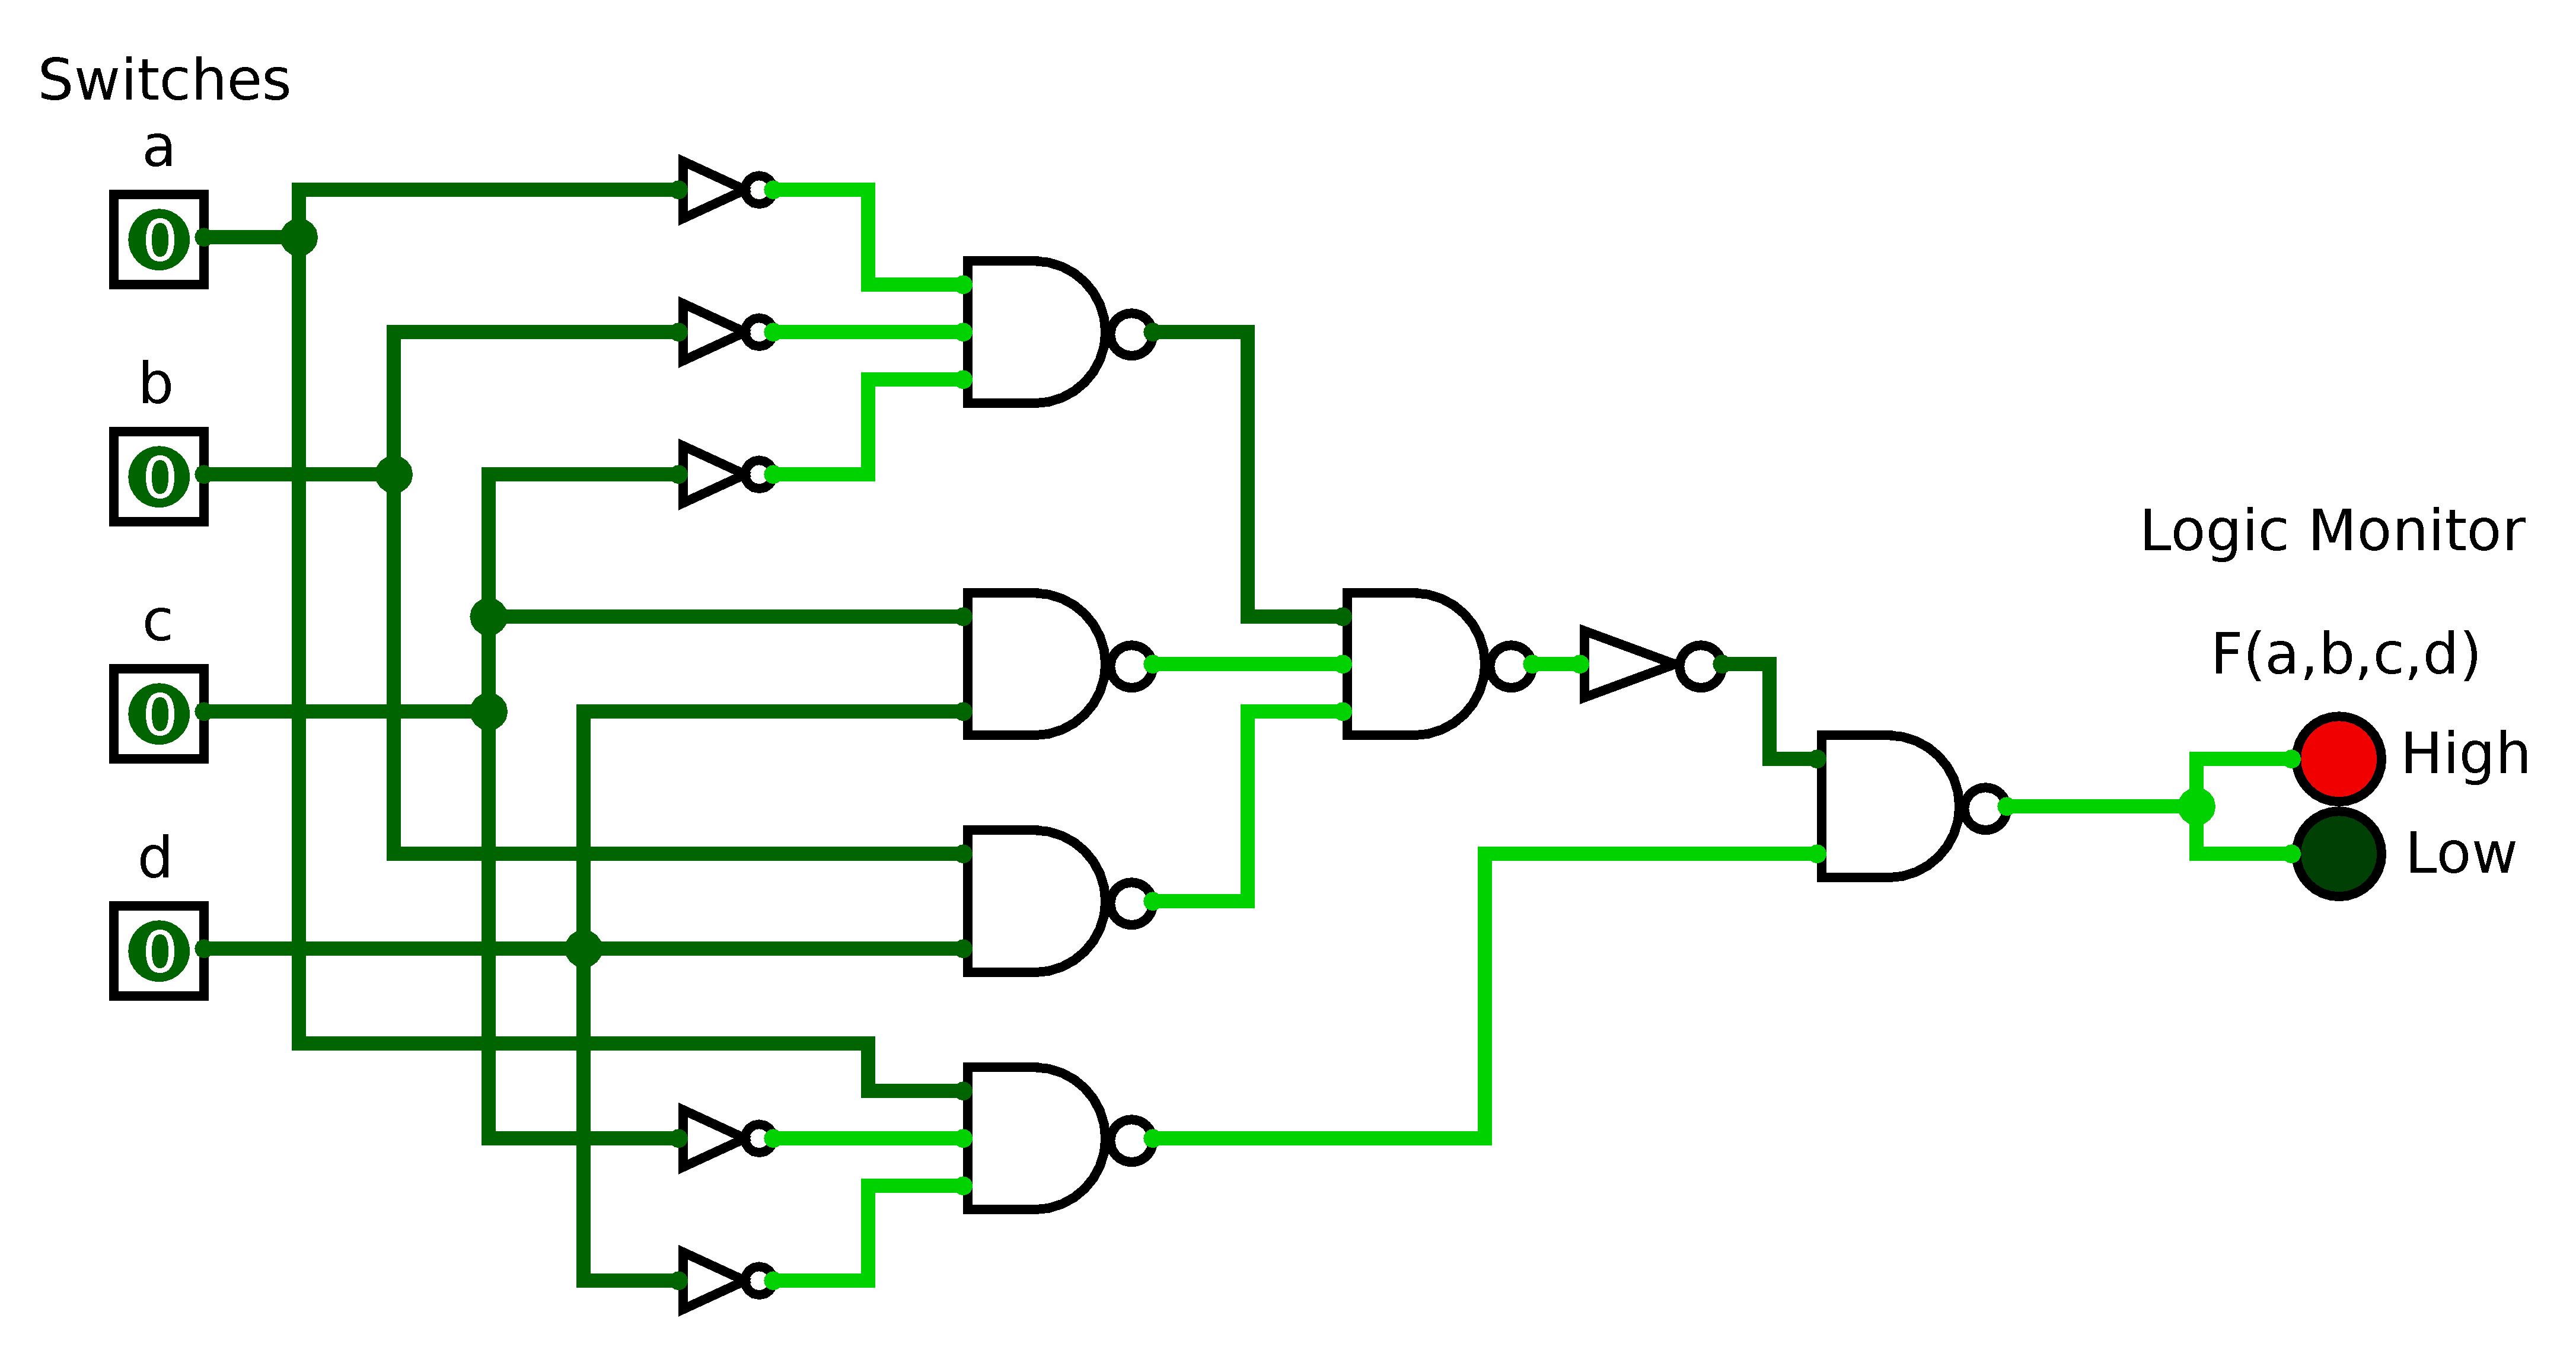
\includegraphics[width=0.5\textwidth]{part2.png}	
	\caption{Circuit of $F$}
	\label{part2}
\end{figure}




\end{flushleft}


\begin{flushleft}
\subsection{PART 3}
\paragraph{}
In the next part of the experiment, the function is designed using a single 8:1 multiplexer and NOT gates. Connections between pins are made for each integrated circuits as needed, outputs are observed on the logic monitor. 


\begin{figure}[!h]
	\centering
	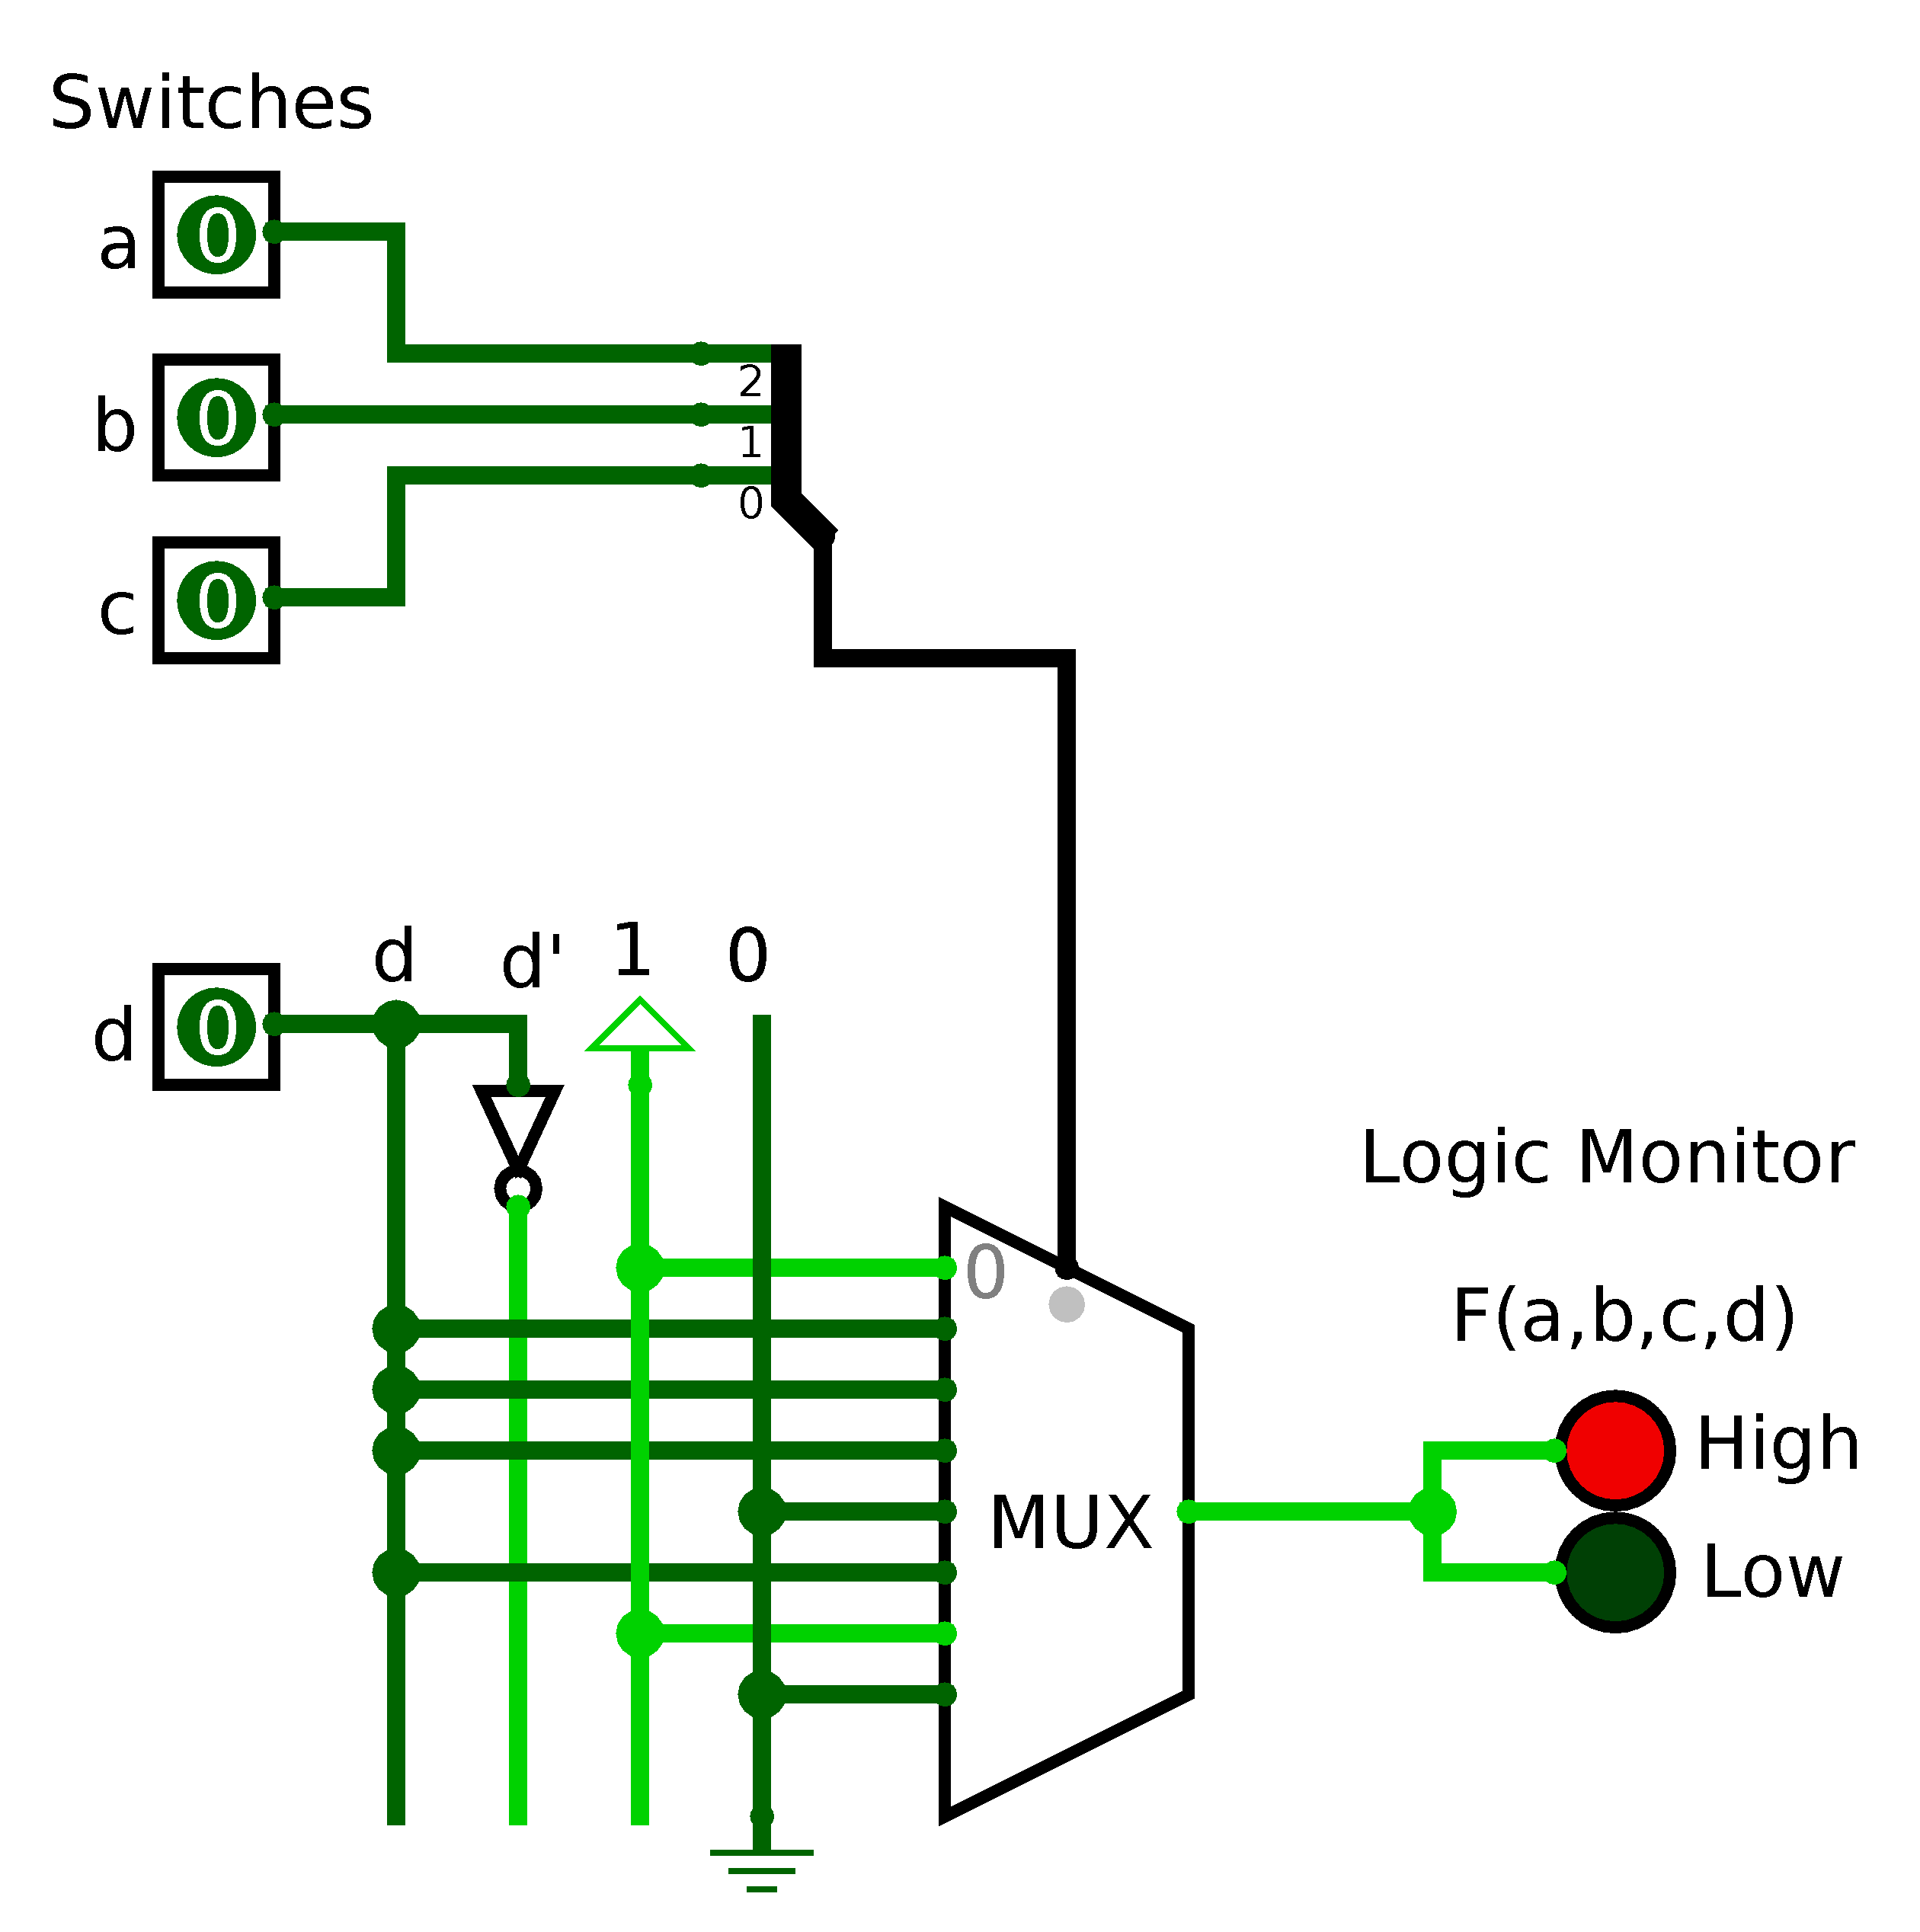
\includegraphics[width=0.5\textwidth]{part3.png}	
	\caption{Circuit of $F$}
	\label{fig1}
\end{figure}

\begin{table}
\centering
    \begin{tabular}{|c|c|c|c|c|c|c|}
    \hline
         A & B & C & D & F &     \\
         \hline
         0 & 0 & 0 & 0 & 1 & \multirow{2}{1em}{1} \\
         0 & 0 & 0 & 1 & ${\Phi}$ & \\
         \hline
         0 & 0 & 1 & 0 & 0 & \multirow{2}{1em}{d}\\
         0 & 0 & 1 & 1 & 1 & \\
         \hline
         0 & 1 & 0 & 0 & 0 & \multirow{2}{1em}{d}\\
         0 & 1 & 0 & 1 & 1 & \\
         \hline
         0 & 1 & 1 & 0 & 0 & \multirow{2}{1em}{d}\\
         0 & 1 & 1 & 1 & 1 & \\
         \hline
         1 & 0 & 0 & 0 & ${\Phi}$ & \multirow{2}{1em}{0} \\
         1 & 0 & 0 & 1 & 0 & \\
         \hline
         1 & 0 & 1 & 0 & 0 & \multirow{2}{1em}{d}\\
         1 & 0 & 1 & 1 & 1 & \\
         \hline
         1 & 1 & 0 & 0 & 1 & \multirow{2}{1em}{1}\\
         1 & 1 & 0 & 1 & 1 & \\
         \hline
         1 & 1 & 1 & 0 & 0 & \multirow{2}{1em}{0}\\
         1 & 1 & 1 & 1 & ${\Phi}$ & \\
         \hline
    \end{tabular}
    \caption{Truth table for multiplexer implementation.}
    \label{truthtablep3}

\end{table}


\paragraph{}
A, B and C input values are connected to the select lines(inputs) of the multiplexer. The remaining D input value is connected according to the truth table above to the data inputs of the multiplexer.

%CIRCUIT








\end{flushleft}
\begin{flushleft}


\subsection{PART 4}
\paragraph{}
In the final part of the experiment, the circuit is designed for the functions below. The circuit is implemented using a single 3:8 decoder, OR, and NOT gates. Connections between pins are made for each integrated circuits as needed, outputs are observed on the logic monitor.


\begin{itemize}
    \item $F_{1}$(a,b,c) = $a' \cdot c'$ + $b \cdot c$          
    \item $F_{2}$(a,b,c) = $a' \cdot b' \cdot c'$ + $a \cdot b$ 
\end{itemize}

\begin{figure}[!h]
	\centering
	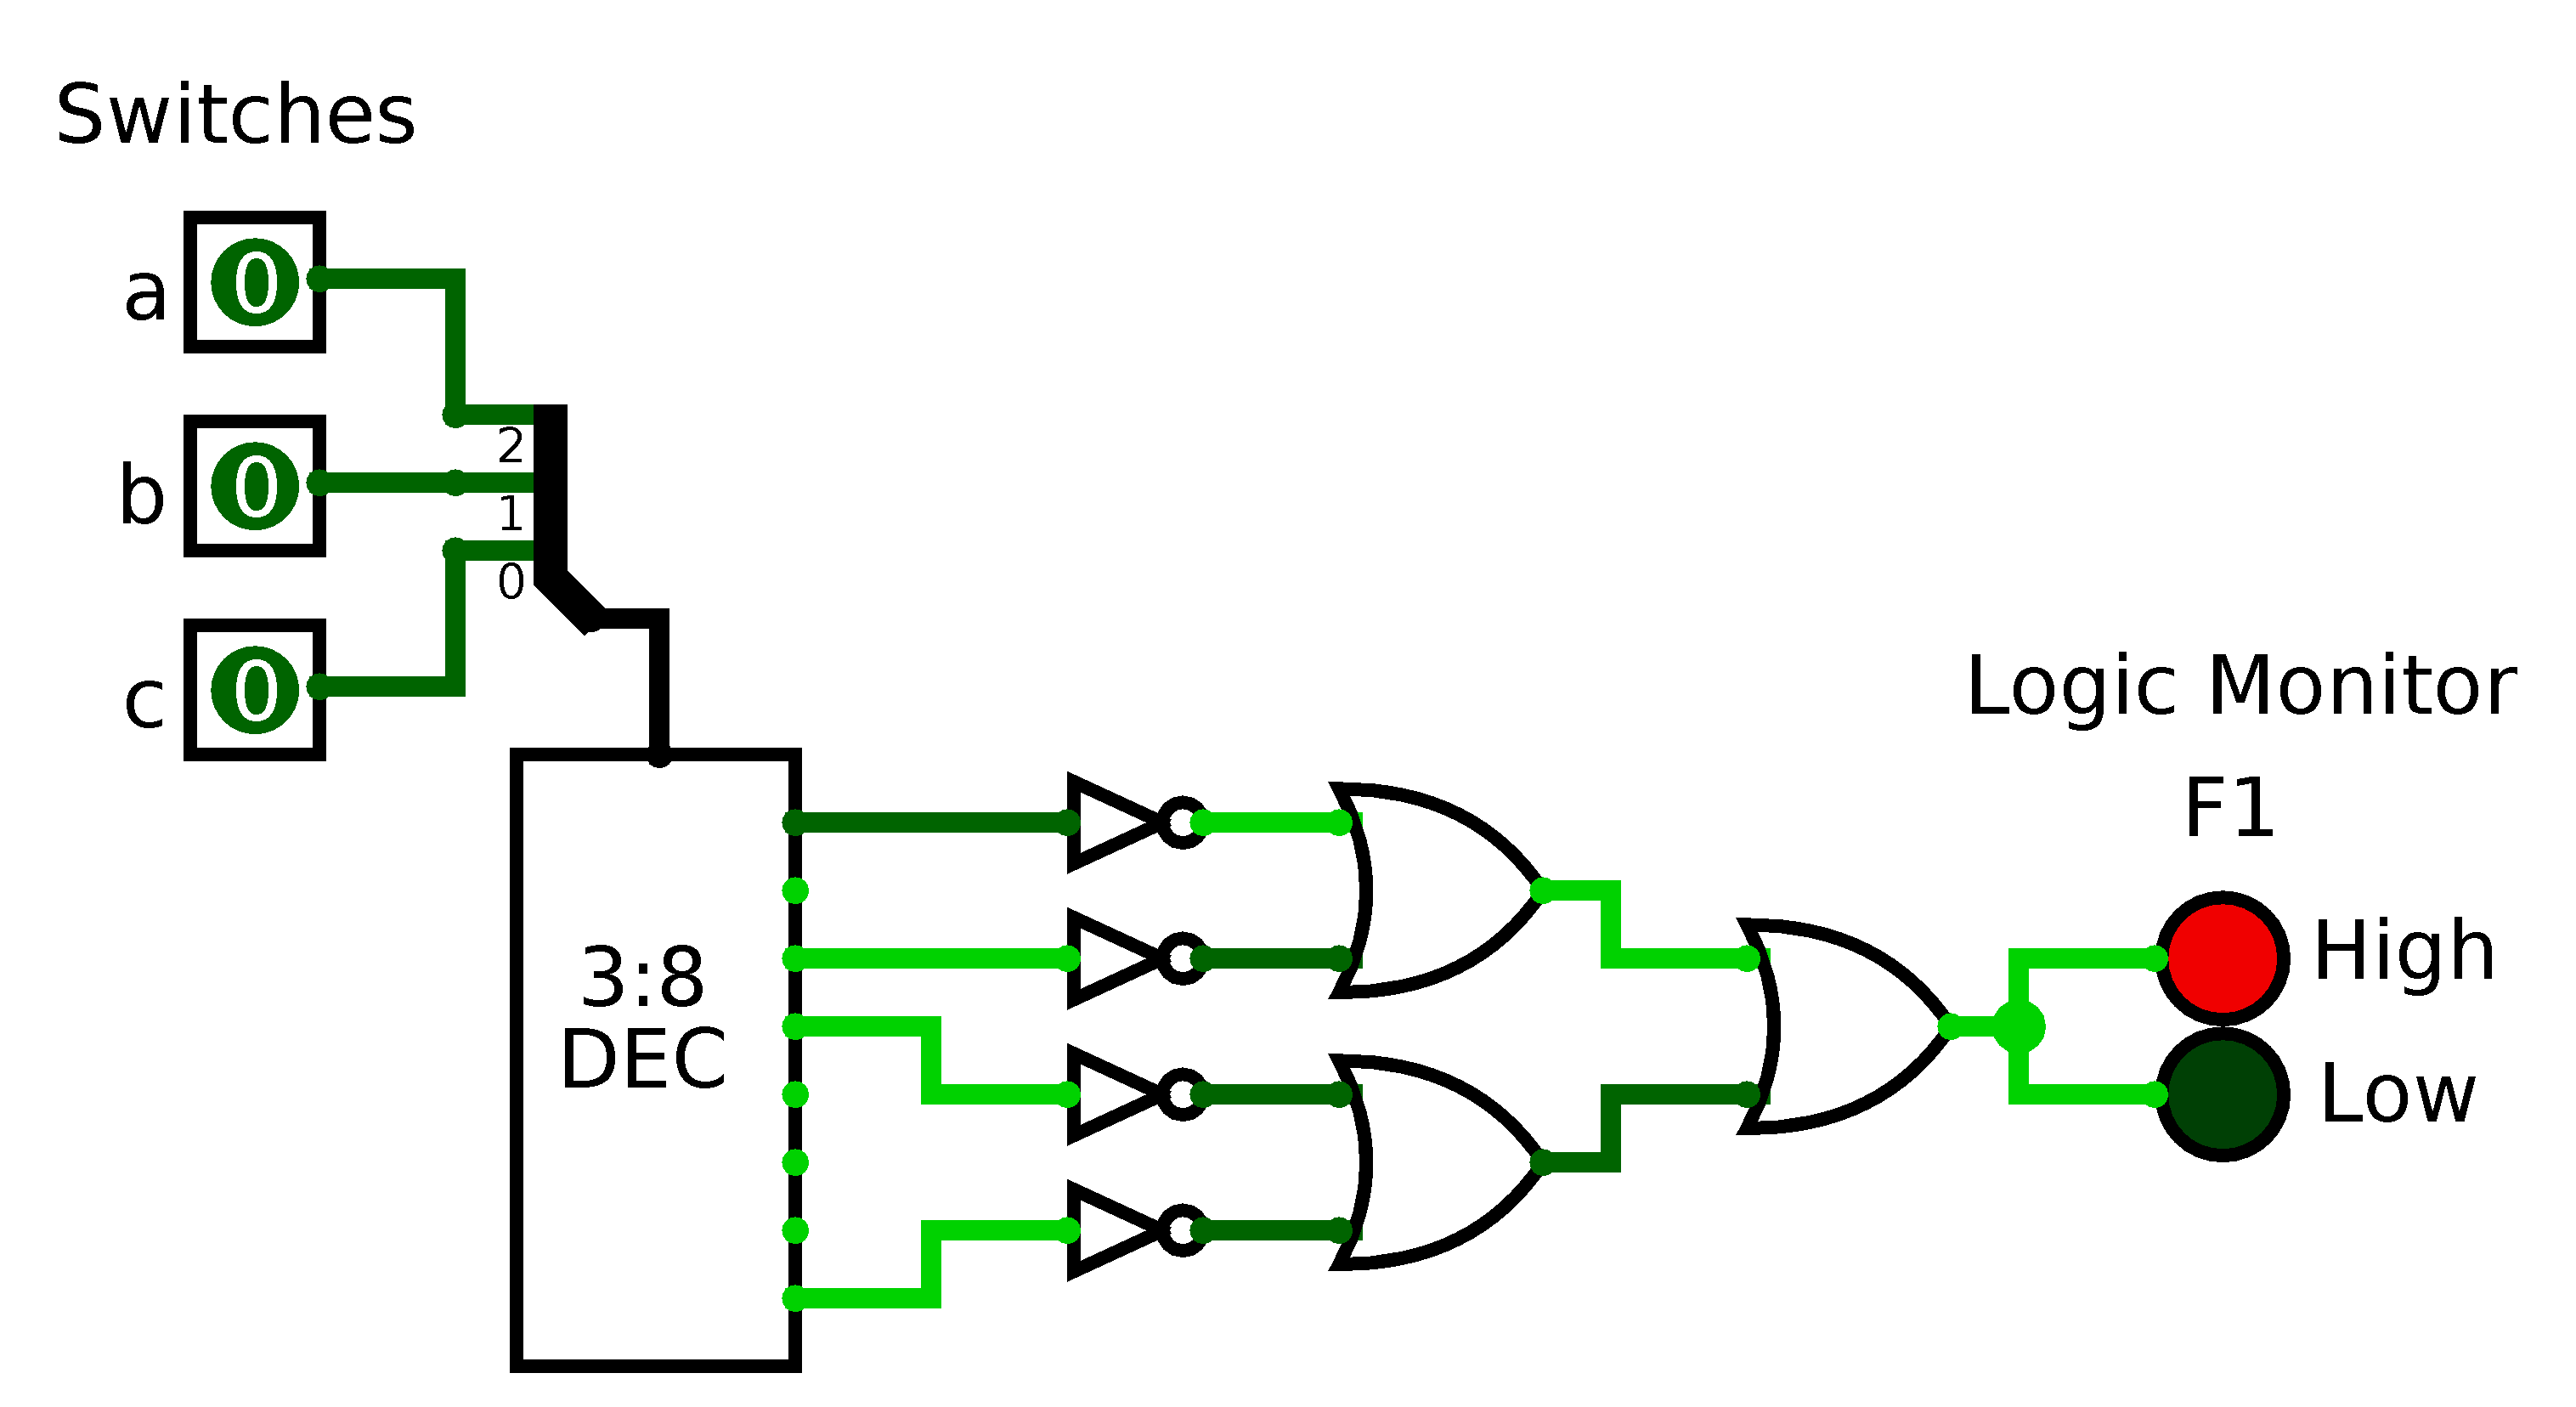
\includegraphics[width=0.5\textwidth]{part4.png}	
	\caption{Circuit of $F_1$}
	\label{fig1}
\end{figure}


\paragraph{}
The first circuit is designed as shown diagram below. The output values in the circuit are validated with the truth table below of the function.

\begin{table}[h]
\centering
\begin{tabular}{|c|c|c|c|c|c|c|c|c|}
\hline
a & b & c & a' & b' & c' & $a' \cdot c'$ & $b \cdot c$ & $F_{1}$ = $a' \cdot c'$ + $b \cdot c$     \\ \hline
0 & 0 & 0 & 1  & 1  & 1  & 1             & 0      & 1             \\ \hline
0 & 0 & 1 & 1  & 1  & 0  & 0             & 0      & 0               \\ \hline
0 & 1 & 0 & 1  & 0  & 1  & 1             & 0      & 1              \\ \hline
0 & 1 & 1 & 1  & 0  & 0  & 0             & 1      & 1               \\ \hline
1 & 0 & 0 & 0  & 1  & 1  & 0             & 0      & 0               \\ \hline
1 & 0 & 1 & 0  & 1  & 0  & 0             & 0      & 0           \\ \hline
1 & 1 & 0 & 0  & 0  & 1  & 0             & 0      & 0          \\ \hline
1 & 1 & 1 & 0  & 0  & 0  & 0             & 1      & 1               \\ \hline
\end{tabular}
\caption{Truth table for F1}
\label{fig3}
\end{table}






\begin{figure}[!h]
	\centering
	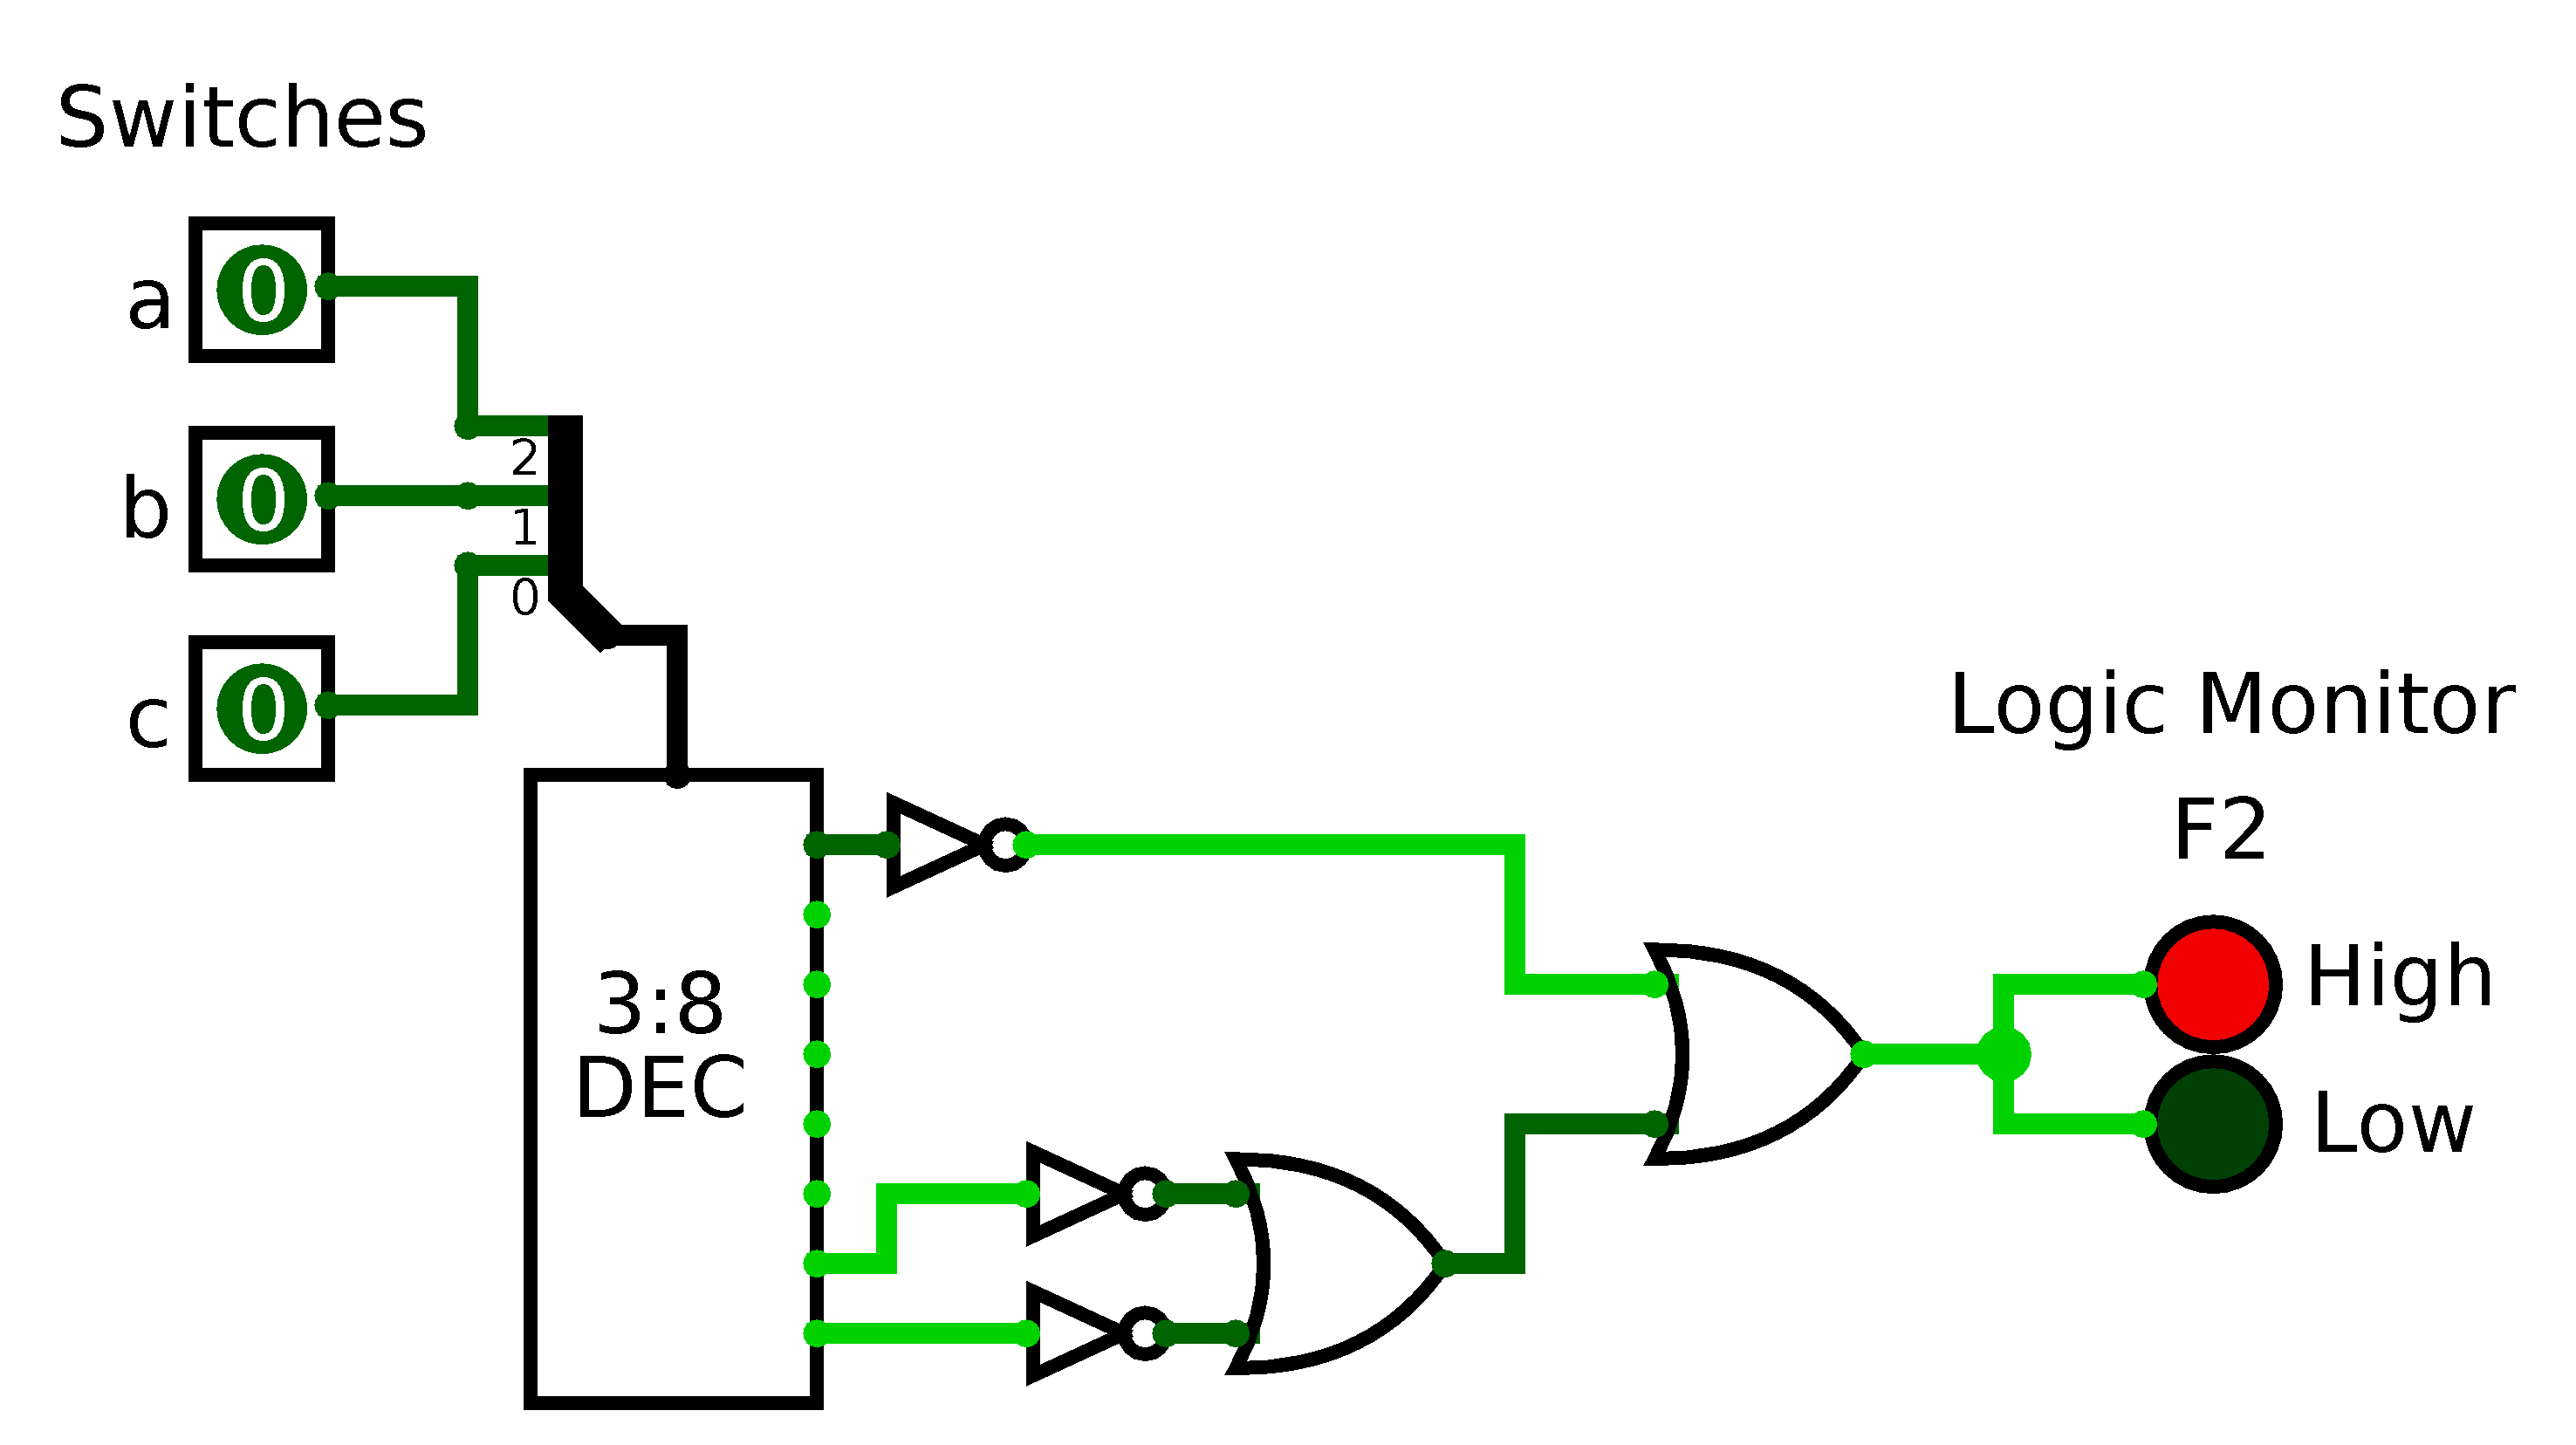
\includegraphics[width=0.5\textwidth]{part4_f2.png}	
	\caption{Circuit of $F_2$}
	\label{fig1}
\end{figure}

\paragraph{}
The second circuit is designed as shown in the diagram(Figure 7). The output values in the circuit are validated with the truth table(Table 7).

\begin{table}[!h]
\centering
\begin{tabular}{|c|c|c|c|c|c|c|c|c|}
\hline
a & b & c & a' & b' & c' & $a' \cdot b' \cdot c'$ & $a \cdot b$ & $F_{2}$ = $a' \cdot b' \cdot c'$ + $a \cdot b$      \\ \hline
0 & 0 & 0 & 1  & 1  & 1  & 1             & 0      & 1             \\ \hline
0 & 0 & 1 & 1  & 1  & 0  & 0             & 0      & 0               \\ \hline
0 & 1 & 0 & 1  & 0  & 1  & 0             & 0      & 0              \\ \hline
0 & 1 & 1 & 1  & 0  & 0  & 0             & 0      & 0               \\ \hline
1 & 0 & 0 & 0  & 1  & 1  & 0             & 0      & 0               \\ \hline
1 & 0 & 1 & 0  & 1  & 0  & 0             & 0      & 0           \\ \hline
1 & 1 & 0 & 0  & 0  & 1  & 0             & 1      & 1          \\ \hline
1 & 1 & 1 & 0  & 0  & 0  & 0             & 1      & 1               \\ \hline
\end{tabular}
\caption{Truth table for F2}
\label{fig3}
\end{table}


\end{flushleft}


\newpage
\section{INTERPRETATION OF THE RESULTS }
\begin{flushleft}
\paragraph{}
We were able to observe the desired-theoretically true results all through the experiment as we were able to figure out the correct designs for the circuits. Results were consistent with the expected result we calculated beforehand. We also faced no equipment failures. Other than the things mentioned above, there wasn't anything worth noting about our results.( Methods used and designs for each circuit have already been explained in detail in part 2 of the report.)

\end{flushleft}



\section{CONCLUSION}
\begin{flushleft}
\paragraph{}
Even though most of the experiment went as expected, there were 2 points where we had to stop and think once more. First of which was part 2 of the experiment where we designed the circuit correctly but made a mistake while implementing it on the cadet unit. But we were able to resolve the issue with the cost being more time than necessary spent on the step. The second point was part 4, where we had to use a decoder. We had a problem figuring out what the inputs should be. But that confusion also didn't last long and we got back on track to finish the experiment as planned.
%aslında hayvan gibi zor olan yanlış fonksiyonu yapmaya çalıştık hayatımız kayıyodu ama onu anlatmıcak çünkü çok saçma

\end{flushleft}
\newpage


\nocite{overleaf}
\nocite{reportGuide}

\addcontentsline{toc}{section}{\numberline {}REFERENCES}


\bibliographystyle{unsrt}
\bibliography{reference}

\end{document}

